\section{Agentic Context Engineering (ACE)}
\label{sec:methods}

We present ACE (\textbf{A}gentic \textbf{C}ontext \textbf{E}ngineering), a framework for scalable and efficient context adaptation in both offline (\eg system prompt optimization) and online (\eg test-time memory adaptation) scenarios. 
Instead of condensing knowledge into terse summaries or static instructions, ACE treats contexts as evolving playbooks that continuously accumulate, refine, and organize strategies over time. 
Inspired by the agentic design of Dynamic Cheatsheet~\citep{suzgun2025dynamic}, ACE introduces a structured division of labor across three roles (Figure \ref{fig:design}): the \emph{Generator}, which produces reasoning trajectories; the \emph{Reflector}, which distills concrete insights from successes and errors; and the \emph{Curator}, which integrates these insights into structured context updates. 
This mirrors how humans learn: experimenting, reflecting, and consolidating, while avoiding the bottleneck of overloading a single model with all responsibilities.  

\begin{figure}[!htbp]
    \centering
    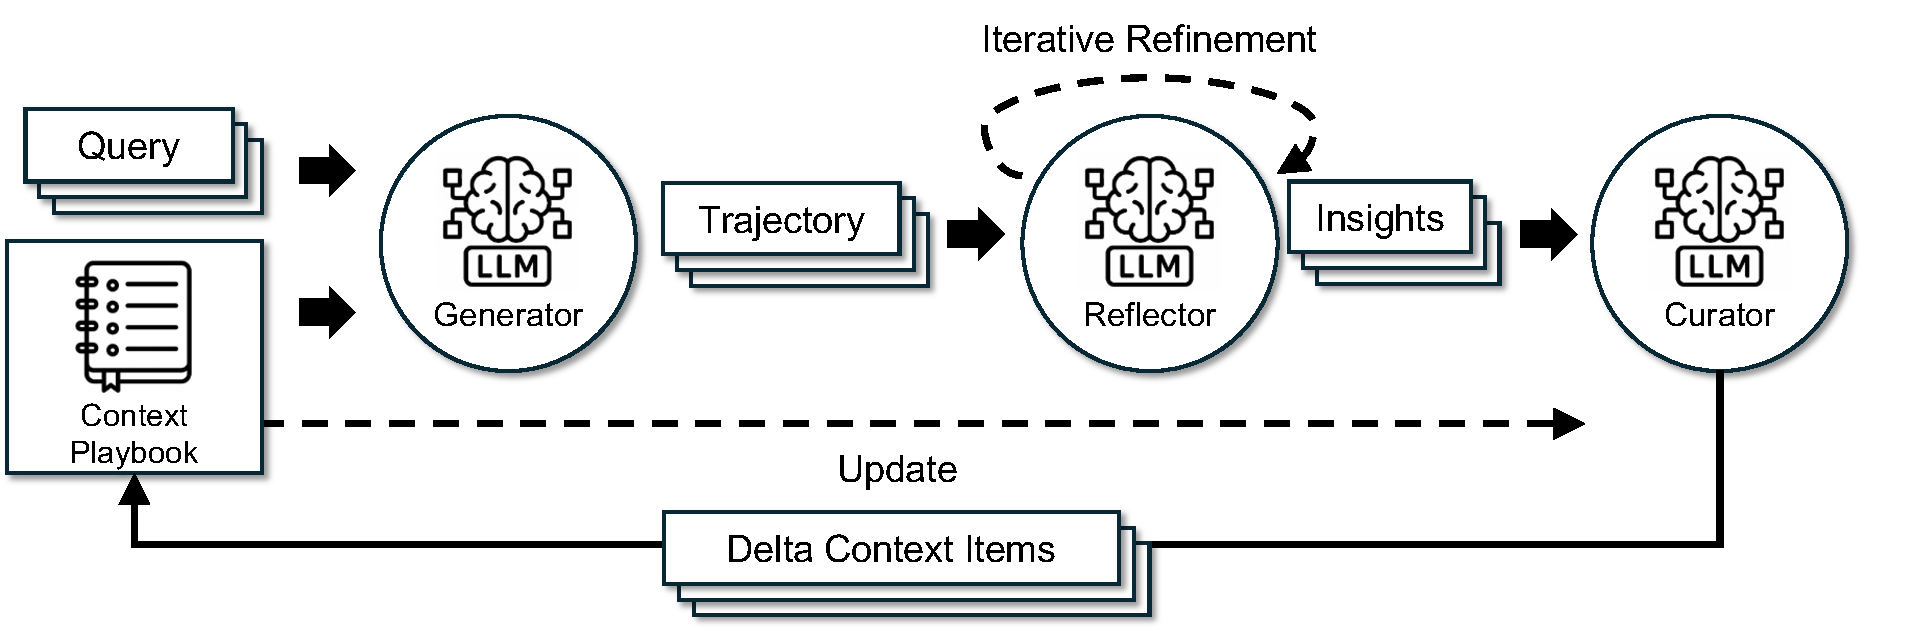
\includegraphics[width=0.95\textwidth]{figures/figure_4_CR.pdf}
    \caption{\textbf{The \name Framework.} Inspired by Dynamic Cheatsheet, ACE adopts an agentic architecture with three specialized components: a Generator, a Reflector, and a Curator.}
    \label{fig:design}
\end{figure}

To address the limitations of prior methods discussed in \S\ref{subsec:limitations} (notably \textit{brevity bias} and \textit{context collapse}) ACE introduces three key innovations:  
(1) a dedicated \textit{Reflector} that separates evaluation and insight extraction from curation, improving context quality and downstream performance (\S\ref{subsec:results-ablation});  
(2) incremental \emph{delta updates} (\S\ref{subsec:delta-update}) that replace costly monolithic rewrites with localized edits, reducing both latency and compute cost (\S\ref{subsec:results-cost-speed}); and  
(3) a \emph{grow-and-refine} mechanism (\S\ref{subsec:grow-and-refine}) that balances steady context expansion with redundancy control.  

As shown in Figure~\ref{fig:design}, the workflow begins with the Generator producing reasoning trajectories for new queries, which surface both effective strategies and recurring pitfalls. 
The Reflector critiques these traces to extract lessons, optionally refining them across multiple iterations. 
The Curator then synthesizes these lessons into compact \emph{delta entries}, which are merged deterministically into the existing context by lightweight, non-LLM logic. 
Because updates are itemized and localized, multiple deltas can be merged in parallel, enabling batched adaptation at scale. 
ACE further supports multi-epoch adaptation, where the same queries are revisited to progressively strengthen the context.  

\subsection{Incremental Delta Updates}
\label{subsec:delta-update}

A core design principle of ACE is to represent context as a collection of \emph{structured, itemized bullets}, rather than a single monolithic prompt. 
The concept of a bullet is similar to the concept of a memory entry in LLM memory frameworks like Dynamic Cheatsheet~\citep{suzgun2025dynamic} and A-MEM~\citep{xu2025mem}, but builds on top of that and consists of (1) \textbf{metadata}, including a unique identifier and counters tracking how often it was marked helpful or harmful; and (2) \textbf{content}, capturing a small unit such as a reusable strategy, domain concept, or common failure mode. 
When solving new problems, the Generator highlights which bullets were useful or misleading, providing feedback that guides the Reflector in proposing corrective updates. 

This itemized design enables three properties: 
(1) \emph{localization}, so only the relevant bullets are updated; 
(2) \emph{fine-grained retrieval}, so the Generator can focus on the most pertinent knowledge; and 
(3) \emph{incremental adaptation}, allowing efficient merging, pruning, and de-duplication during inference.

Rather than regenerating contexts in full, ACE incrementally produces compact \emph{delta contexts}: small sets of candidate bullets distilled by the Reflector and integrated by the Curator. 
This avoids the computational cost and latency of full rewrites, while ensuring that past knowledge is preserved and new insights are steadily appended. 
As contexts grow, this approach provides the scalability needed for long-horizon or domain-intensive applications.

\subsection{Grow-and-Refine}
\label{subsec:grow-and-refine}

Beyond incremental growth, ACE ensures that contexts remain compact and relevant through periodic or lazy refinement. 
In grow-and-refine, bullets with new identifiers are appended, while existing bullets are updated in place (\eg incrementing counters). 
A de-duplication step then prunes redundancy by comparing bullets via semantic embeddings. 
This refinement can be performed proactively (after each delta) or lazily (only when the context window is exceeded), depending on application requirements for latency and accuracy.

Together, incremental updates and grow-and-refine maintain contexts that expand adaptively, remain interpretable, and avoid the potential variance introduced by monolithic context rewriting.